\hypertarget{_mesh_renderer_8cpp}{}\section{Mesh\+Renderer.\+cpp File Reference}
\label{_mesh_renderer_8cpp}\index{Mesh\+Renderer.\+cpp@{Mesh\+Renderer.\+cpp}}
{\ttfamily \#include \char`\"{}Mesh\+Renderer.\+h\char`\"{}}\newline
{\ttfamily \#include \char`\"{}Vertex\+Array.\+h\char`\"{}}\newline
{\ttfamily \#include \char`\"{}Vertex\+Buffer.\+h\char`\"{}}\newline
{\ttfamily \#include \char`\"{}Shader\+Program.\+h\char`\"{}}\newline
{\ttfamily \#include \char`\"{}Transform.\+h\char`\"{}}\newline
{\ttfamily \#include \char`\"{}Screen.\+h\char`\"{}}\newline
{\ttfamily \#include \char`\"{}Core.\+h\char`\"{}}\newline
{\ttfamily \#include \char`\"{}Entity.\+h\char`\"{}}\newline
{\ttfamily \#include \char`\"{}Camera.\+h\char`\"{}}\newline
{\ttfamily \#include \char`\"{}Resources.\+h\char`\"{}}\newline
{\ttfamily \#include $<$gtc\textbackslash{}matrix\+\_\+transform.\+hpp$>$}\newline
{\ttfamily \#include $<$iostream$>$}\newline
Include dependency graph for Mesh\+Renderer.\+cpp\+:
\nopagebreak
\begin{figure}[H]
\begin{center}
\leavevmode
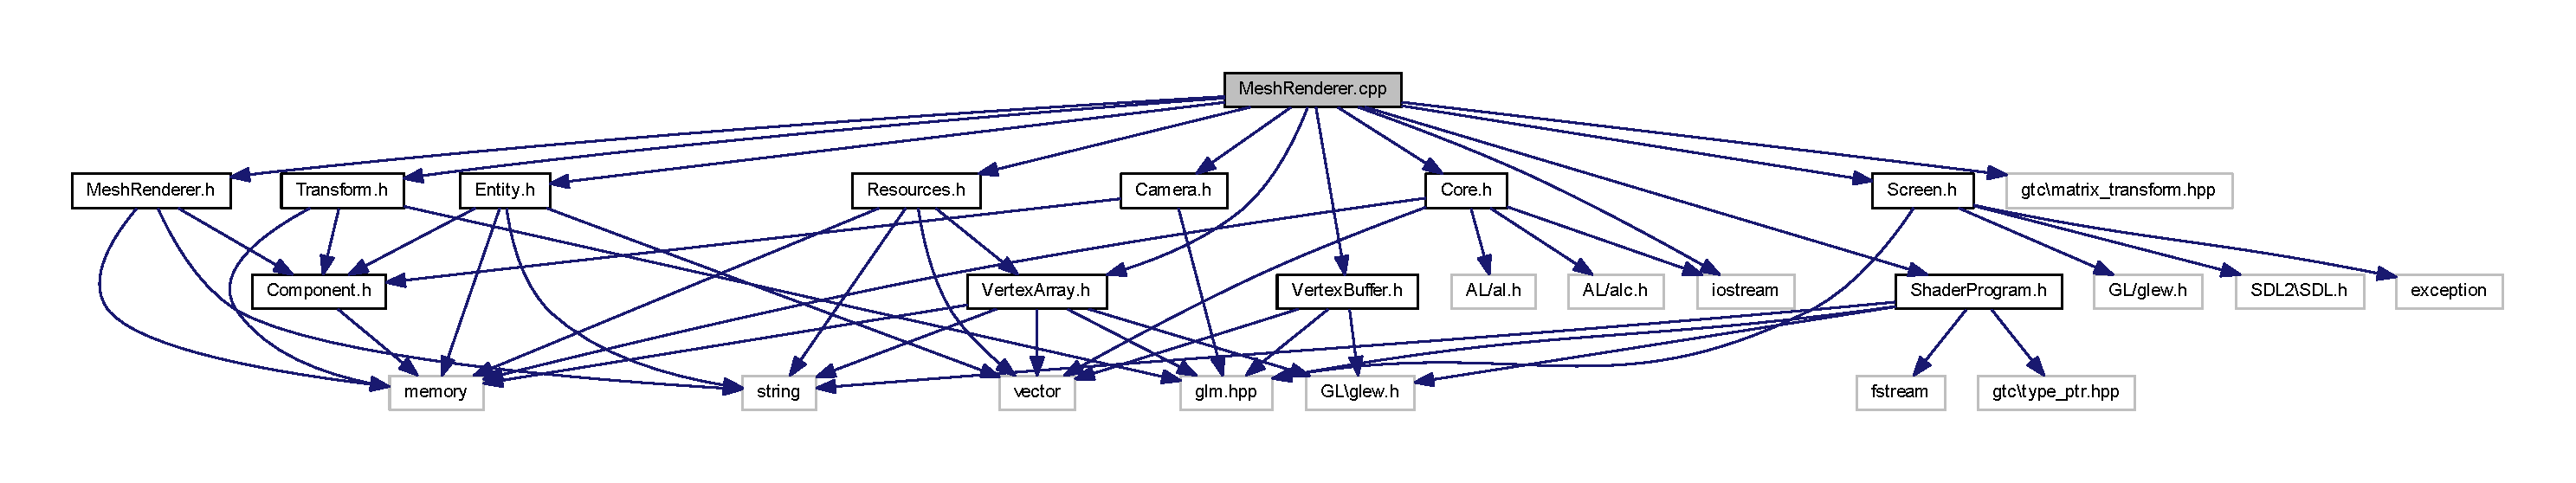
\includegraphics[width=350pt]{_mesh_renderer_8cpp__incl}
\end{center}
\end{figure}
